\documentclass{standalone}
\usepackage{tikz}
\usetikzlibrary{calc}
\begin{document}
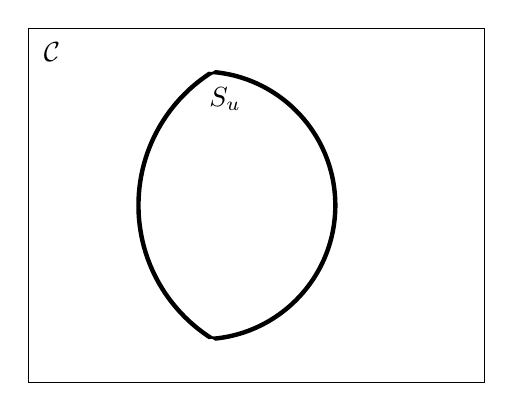
\begin{tikzpicture}

\ifdefined\argstart
   \def\drawrightspec{}
\fi
\ifdefined\argroadmap
   \def\drawroadmap{}
   \def\drawrightspec{}
\fi
\ifdefined\argstraightsol
   \def\drawroadmap{}
   \def\drawrightspec{}
   \def\drawstraightsol{}
\fi

\ifdefined\argbasesets
   \def\drawroadmap{}
   \def\drawbasesets{}
   \def\drawrightspec{}
\fi
\ifdefined\argblackgraph
   \def\drawroadmap{}
   \def\drawbasesets{}
   \def\drawblackgraph{}
   \def\drawrightspec{}
\fi

\ifdefined\argrightsol
   \def\drawroadmap{}
   \def\drawbasesets{}
   \def\drawblackgraph{}
   \def\drawrightspec{}
   \def\drawrightsol{}
\fi

\ifdefined\argleftspec
   \def\drawroadmap{}
   \def\drawbasesets{}
   \def\drawblackgraph{}
   \def\drawleftspec{}
\fi
\ifdefined\argleftsol
   \def\drawroadmap{}
   \def\drawbasesets{}
   \def\drawblackgraph{}
   \def\drawleftspec{}
   \def\drawleftsol{}
\fi

% original problem spec
%\def\drawrightspec{}
%\def\drawrightsol{}
%\def\drawleftspec{}
%\def\drawleftsol{}

%\def\drawblackgraph{}
%\def\drawbasesets{}

%\begin{scope}[shift={(2.2,2.45)}]
%\draw[step=1,black!10,very thin] (-1,-1) grid (1,1);
%\end{scope}

\draw (0,0.2) rectangle (5.8,4.7);

\coordinate (r) at (2.2,2.45);
\coordinate (e) at (3.4,2.45);

\def\circler{(r) circle (1.7)}
\def\circlee{(e) circle (2.0)}

\node (clab) at (0.3,4.4) {$\mathcal{C}$};
\node (flab) at (2.5,3.8) {$S_u$};

\coordinate (v01) at ($ (r) + (-1.10, 0.70) $);
\coordinate (v02) at ($ (r) + (-1.10,-0.86) $);
\coordinate (v03) at ($ (r) + (-1.00,-0.19) $);
\coordinate (v04) at ($ (r) + (-0.50,-0.40) $);
\coordinate (v05) at ($ (r) + (-0.30, 0.41) $);
\coordinate (v07) at ($ (r) + ( 0.30,-1.20) $);
\coordinate (v08) at ($ (r) + ( 0.16, 0.28) $);
\coordinate (v09) at ($ (r) + ( 0.38,-0.64) $);
\coordinate (v06) at ($ (r) + ( 0.40, 0.90) $);
\coordinate (v10) at ($ (r) + ( 0.90, 0.20) $);
\coordinate (v11) at ($ (r) + ( 0.99,-0.32) $);
\coordinate (v12) at ($ (r) + ( 1.33,-0.30) $);
\coordinate (v13) at ($ (r) + (-0.70, 1.10) $);
\coordinate (v14) at ($ (r) + (1.80, 0.60) $);
\coordinate (v15) at ($ (r) + (1.60, -1.00) $);
\coordinate (q1) at ($ (r) + (0.9, 1.1) $);
\coordinate (q2) at ($ (r) + (0.8,-1.2) $);
\coordinate (q3) at ($ (r) + (-0.2, 1.2) $);
\coordinate (q4) at ($ (r) + (-0.4, -1.0) $);

\ifdefined\drawstraightsol
   \draw[color=black!20,line width=7,line cap=round]
      (q2) -- (v11) -- (v10) -- (q1);
\fi
\ifdefined\drawrightsol
   \draw[color=black!20,line width=7,line cap=round]
      (q2) -- (v07) -- (v09) -- (v08) -- (v06) -- (q1);
\fi
\ifdefined\drawleftsol
   \draw[color=black!20,line width=7,line cap=round]
      (q4) -- (v04) -- (v03) -- (v01) -- (v13) -- (q3);
\fi

% XnY
\begin{scope}
   \clip \circler;
   %\fill[pattern=horizontal lines] \circley;
   \draw[ultra thick] \circlee;
\end{scope}
\begin{scope}
   \clip \circlee;
   \draw[ultra thick] \circler;
\end{scope}
\ifdefined\drawbasesets
   \draw[dashed] \circler;
   \draw[dashed] \circlee;
   \node (rlab) at ($ (r) + (-1.4,0) $) {$S_A$};
   \node (elab) at ($ (e) + ( 1.7,0) $) {$S_B$};
\fi

\ifdefined\drawroadmap
   \node[circle,fill=black,inner sep=1.0] at (v01) {};
   \node[circle,fill=black,inner sep=1.0] at (v02) {};
   \node[circle,fill=black,inner sep=1.0] at (v03) {};
   \node[circle,fill=black,inner sep=1.0] at (v04) {};
   \node[circle,fill=black,inner sep=1.0] at (v05) {};
   \node[circle,fill=black,inner sep=1.0] at (v07) {};
   \node[circle,fill=black,inner sep=1.0] at (v08) {};
   \node[circle,fill=black,inner sep=1.0] at (v09) {};
   \node[circle,fill=black,inner sep=1.0] at (v06) {};
   \node[circle,fill=black,inner sep=1.0] at (v10) {};
   \node[circle,fill=black,inner sep=1.0] at (v11) {};
   \node[circle,fill=black,inner sep=1.0] at (v12) {};
   \node[circle,fill=black,inner sep=1.0] at (v13) {};
   \node[circle,fill=black,inner sep=1.0] at (v14) {};
   \node[circle,fill=black,inner sep=1.0] at (v15) {};
   \node[circle,fill=black,inner sep=1.0] at (q1) {};
   \node[circle,fill=black,inner sep=1.0] at (q2) {};
   \node[circle,fill=black,inner sep=1.0] at (q3) {};
   \node[circle,fill=black,inner sep=1.0] at (q4) {};
   
   % dotted underneath
   \draw[color=black,dotted] (v01) -- (v03) -- (v02) -- (v04) -- (v03);
   \draw[color=black,dotted] (v01) -- (v05) -- (v04) -- (v07) -- (v09) -- (v04);
   \draw[color=black,dotted] (v04) -- (v08) -- (v05) -- (v06) -- (v08) -- (v10);
   \draw[color=black,dotted] (v08) -- (v09) -- (v11) -- (v10);
   \draw[color=black,dotted] (v11) -- (v12) -- (v10);
   \draw[color=black,dotted] (v11) -- (v12) -- (v10);
   \draw[color=black,dotted] (v01) -- (v13) -- (v05);

   \draw[color=black,dotted] (v06) -- (q1) -- (v10);
   \draw[color=black,dotted] (v07) -- (q2) -- (v09);
   \draw[color=black,dotted] (q2) -- (v11);
   \draw[color=black,dotted] (v13) -- (q3) -- (v05);
   \draw[color=black,dotted] (q3) -- (v06);
   \draw[color=black,dotted] (v02) -- (q4) -- (v04);
   \draw[color=black,dotted] (v02) -- (q4) -- (v07);
   \draw[color=black,dotted] (q1) -- (v14) -- (v10);
   \draw[color=black,dotted] (v14) -- (v12);
   \draw[color=black,dotted] (v12) -- (v15) -- (q2);
\fi

% dotted underneath
\ifdefined\drawblackgraph
   \draw (v01) -- (v03) -- (v02) -- (v04) -- (v03);
   \draw (v01) -- (v05) -- (v04) -- (v07) -- (v09) -- (v04);
   \draw (v04) -- (v08) -- (v05) -- (v06) -- (v08) -- (v10);
   \draw (v08) -- (v09) -- (v11) -- (v10);
   \draw (v11) -- (v12) -- (v10);
   \draw (v11) -- (v12) -- (v10);
   \draw (v01) -- (v13) -- (v05);
\fi

\ifdefined\drawrightspec
   \node[circle,fill=black,inner sep=1.5] (q1node) at (q1) {};
   \node[circle,fill=black,inner sep=1.5] (q2node) at (q2) {};
   \node (q1lab) at (4.1,3.7) {$q_{\mbox{\scriptsize init}}$};
   \node (q2lab) at (4.0,1.0) {$q_{\mbox{\scriptsize goal}}$};
   \draw[->] (q1lab) -- (q1node);
   \draw[->] (q2lab) -- (q2node);
\fi

\ifdefined\drawleftspec
   \node[circle,fill=black,inner sep=1.5] (q3node) at (q3) {};
   \node[circle,fill=black,inner sep=1.5] (q4node) at (q4) {};
   \node (q3lab) at (1.7,4.4) {$q_{\mbox{\scriptsize init}}$};
   \node (q4lab) at (1.6,0.5) {$q_{\mbox{\scriptsize goal}}$};
   \draw[->] (q3lab) -- (q3node);
   \draw[->] (q4lab) -- (q4node);
\fi

\end{tikzpicture}%
\end{document}
